\documentclass[10pt,t]{beamer}
\usetheme{desynew}

\usepackage[utf8]{inputenc}
\usepackage[T1]{fontenc}
\usepackage{textcomp}
\usepackage[ngerman]{babel}
\usepackage{microtype}
\usepackage{hyperref}

%%%
%%%  Grafik

\usepackage{tikz}
\usetikzlibrary{positioning,calc}
%%% enable grid for finding text positions
%\usepackage[texcoord,grid,gridunit=mm,gridcolor=red!10,subgridcolor=green!10]{eso-pic}

%%%
%%%  Bibliography
%%%

\usepackage[backend=biber,style=numeric,sorting=none]{biblatex}
\setbeamertemplate{bibliography item}{\insertbiblabel} % sonst stehen da Icons statt der Zitat-Abkürzung
\renewcommand*{\bibfont}{\tiny}
\usepackage{csquotes}
\addbibresource{references.bib}

%%%
%%%  Dokumenteneinstellungen
%%%

\title[Willkommen am DESY]{Willkommen am DESY!}
\author[Stefan May]{\textbf{Stefan May}}
\institute{Softwareentwickler und Strahlenschutzbeauftragter\\Gruppe MPS (Maschine Personensicherheit)\\[\baselineskip]Einführungsvortrag}
\date[März 2020]{März 2020}

\def\Put(#1,#2)#3{\leavevmode\makebox(0,0){\put(#1,#2){#3}}}
\unitlength=0.01\paperwidth


\begin{document}

\maketitle

\section{Was ist DESY?}

\begin{frame}
\frametitle{Was ist DESY?}
\vspace*{-2\baselineskip}
\begin{columns}[c]
\column{0.472\textwidth}\begin{itemize}
    \item \textbf{D}eutsches \textbf{E}lektronen-\textbf{Sy}nchrotron
    \item Nationales Forschungszentrum
    \item Mitglied der Helmholtz-Gemeinschaft
    \item gegründet am 18. Dezember 1959
    \item Standorte in
    \begin{itemize}
        \item Hamburg
        \item Zeuthen (Brandenburg)
    \end{itemize}
    \item Budget: 230 Million Euro (2016)
    \begin{itemize}
        \item 90\,\% Bundesministerium für Bildung und Forschung (BmBF)
        \item 10\,\% Bundesländer Hamburg und Brandenburg
    \end{itemize}
\end{itemize}
\column{0.472\textwidth}
    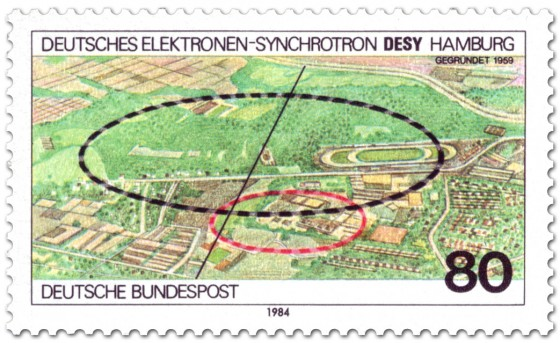
\includegraphics[width=\textwidth]{briefmarke} \\[1ex]
    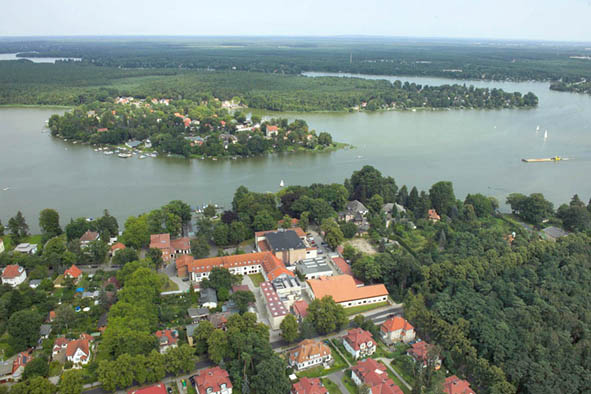
\includegraphics[width=\textwidth]{zeuthen}
\end{columns}
\end{frame}


\begin{frame}
\frametitle{Helmholtz-Gemeinschaft}
\framesubtitle{Helmholtz-Gemeinschaft Deutscher Forschungszentren}
\vspace*{-1.5\baselineskip}
\begin{itemize}
    \item größte Wissenschaftsorganisation Deutschlands
    \begin{itemize}
        \item mehr als 39.0000 Mitarbeiter*innen in 19 Forschungszentren
        \item Budget: 4,5 Milliarden Euro, davon 30\% Drittmittel (2018)
    \end{itemize}
    \item langfristige Grundlagenforschung zur Lösung froßer und drängender Fragen von Gesellschaft, Wissenschaft und Wirtschaft
    \item Forschungsbereiche:
\end{itemize}

\begin{tikzpicture}
    \node [inner sep=0pt] at (0,0) {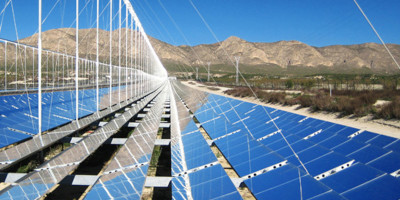
\includegraphics[width=0.3\textwidth]{fb-energie}};
    \node [inner sep=0pt] at (0.35\textwidth,0) {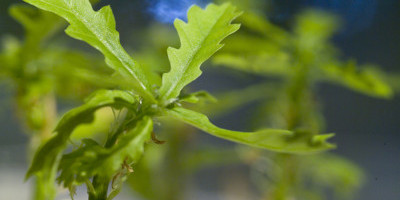
\includegraphics[width=0.3\textwidth]{fb-erdeumwelt}};
    \node [inner sep=0pt] at (0.7\textwidth,0) {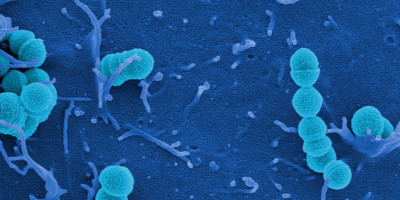
\includegraphics[width=0.3\textwidth]{fb-gesundheit}};
    \node [inner sep=0pt] at (0,-0.2\textwidth) {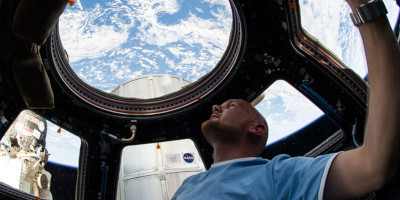
\includegraphics[width=0.3\textwidth]{fb-luftfahrtraumfahrtverkehr}};
    \node [inner sep=0pt] at (0.35\textwidth,-0.2\textwidth) {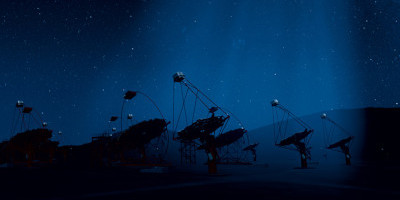
\includegraphics[width=0.3\textwidth]{fb-materie}};
    \node [inner sep=0pt] at (0.7\textwidth,-0.2\textwidth) {
\includegraphics[width=0.3\textwidth]{fb-schluesseltechnologien}};
    \node [fill=desyorange] at (0,0) {\bfseries Energie\vphantom{t}};
    \node [fill=desyorange] at (0.35\textwidth,0) {\bfseries Erde \& Umwelt};
    \node [fill=desyorange] at (0.7\textwidth,0) {\bfseries Gesundheit};
    \node [fill=desyorange] at (0,-0.2\textwidth) {\bfseries\parbox{0.16\textwidth}{\centering Luftfahrt, Raumfahrt, Verkehr}};
    \node [fill=desyorange] at (0.35\textwidth,-0.2\textwidth) {\bfseries Materie};
    \node [fill=desyorange] at (0.7\textwidth,-0.2\textwidth) {\bfseries\parbox{0.19\textwidth}{\centering Schlüssel-technologien}};
\end{tikzpicture}
\end{frame}


\begin{frame}
\frametitle{Menschen am DESY}
\vspace*{-2\baselineskip}
\begin{columns}[c]
\column{0.472\textwidth}\begin{itemize}
    \item etwa 2300 Mitarbeiter
    \begin{itemize}
        \item[$\approx\!$] 650 Wissenschaftler
        \item[$\approx\!$] 700 Studenten, Doktoranden, Postdocs
        \item[$\approx\!$] 100 Auszubildende in technischen und kaufmännischen Berufen
        \item Technik, Verwaltung, \dots
    \end{itemize}
    \item mehr als 3000 Gastwissenschaftler aus 40 Nationen pro Jahr
    \item DESY arbeitet eng mit vielen Hochschulen und anderen Forschungszentren zusammen
    \item DESY betreibt zwei Schülerlabore, um Schüler*innen Wissenschaft näherzubringen
\end{itemize}
\column{0.472\textwidth}
    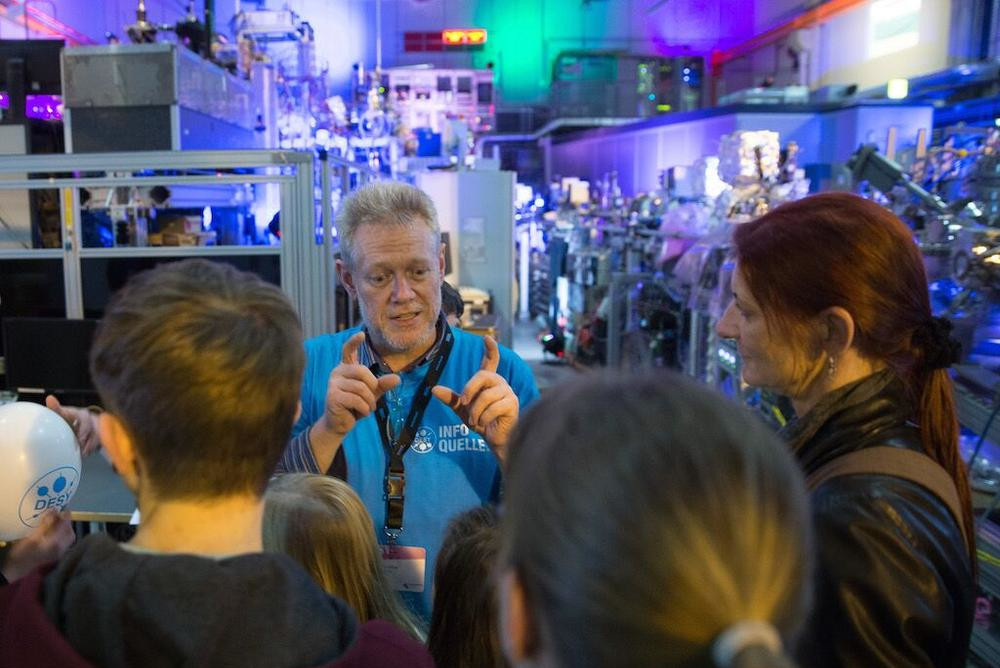
\includegraphics[width=\textwidth]{menschen3} \\[1ex]
    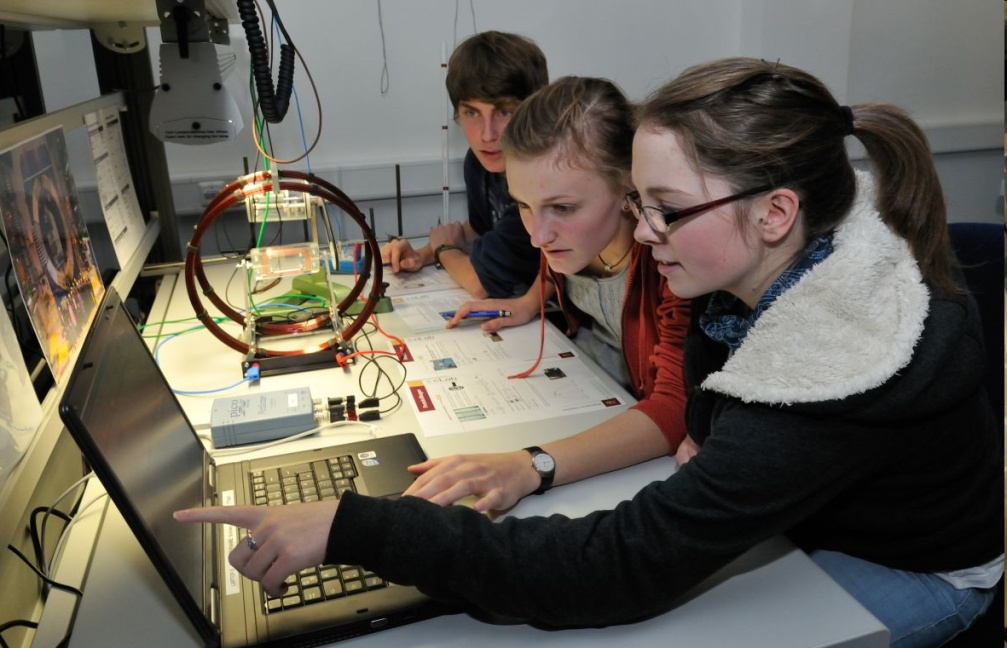
\includegraphics[width=\textwidth]{menschen1} \vspace*{-1cm}
\end{columns}
\end{frame}


\begin{frame}\raggedleft
\frametitle{DESY Campus in Hamburg}
\vspace*{-3.5\baselineskip}
\begin{tikzpicture}
    \node [inner sep=0pt] {\includegraphics[width=0.72\textwidth]{gelaendeplan-hamburg}};
    \node [inner sep=2pt,fill=white] (cfel) at (5.7cm,4cm) {
\includegraphics[width=2cm]{logo-cfel}};
    \node [inner sep=2pt,fill=white,below=0.3cm of cfel] (embl) {
\includegraphics[width=2cm]{logo-embl}};
    \node [inner sep=2pt,fill=white,below=0.3cm of embl] (uhh) {
\includegraphics[width=2cm]{logo-uhh}};
    \node [inner sep=2pt,fill=white,below=0.3cm of uhh] (mpsd) {
\includegraphics[width=2cm]{logo-mpsd}};
    \node [inner sep=2pt,fill=white,below=0.3cm of mpsd] (cssb) {
\includegraphics[width=2cm]{logo-cssb}};
    \node [inner sep=2pt,fill=white,below=0.3cm of cssb] (hzg) {
\includegraphics[width=2cm]{logo-hzg-english}};
    \node [inner sep=2pt,fill=white,below=0.3cm of hzg] (pier) {
\includegraphics[width=2cm]{logo-pier-english}};
    \draw [ultra thick,desyorange,->] (cfel.west) -- (2.6cm,2.3cm);
    \draw [ultra thick,desyorange,->] (embl.west) -- (2.1cm,0.8cm);
    \draw [ultra thick,desyorange,->] (uhh.west) -- (3.5cm,0.5cm);
    \draw [ultra thick,desyorange,->] ($(mpsd.west)!0.2!(mpsd.south west)$) -- (2.8cm,0.2cm);
    \draw [ultra thick,desyorange,->] (cssb.west) -- (1.9cm,0.1cm);
    \draw [ultra thick,desyorange,->] ($(hzg.west)!0.2!(hzg.north west)$) -- (2.6cm,-0.4cm);
    \draw [ultra thick,desyorange,->] ($(pier.west)!0.4!(pier.north west)$) -- (2.2cm,-0.55cm);
    \node [inner sep=0pt] at (-3.5cm,-2.8cm) {\includegraphics[width=0.1\textwidth]{logos/desy}};
\end{tikzpicture}
\vspace*{-13pt}
\end{frame}

\section{Forschung am DESY}

\begin{frame}
\frametitle{Forschung am DESY}
\vspace*{-2\baselineskip}
\begin{tikzpicture}
    \node[inner sep=0pt] at (0,0) {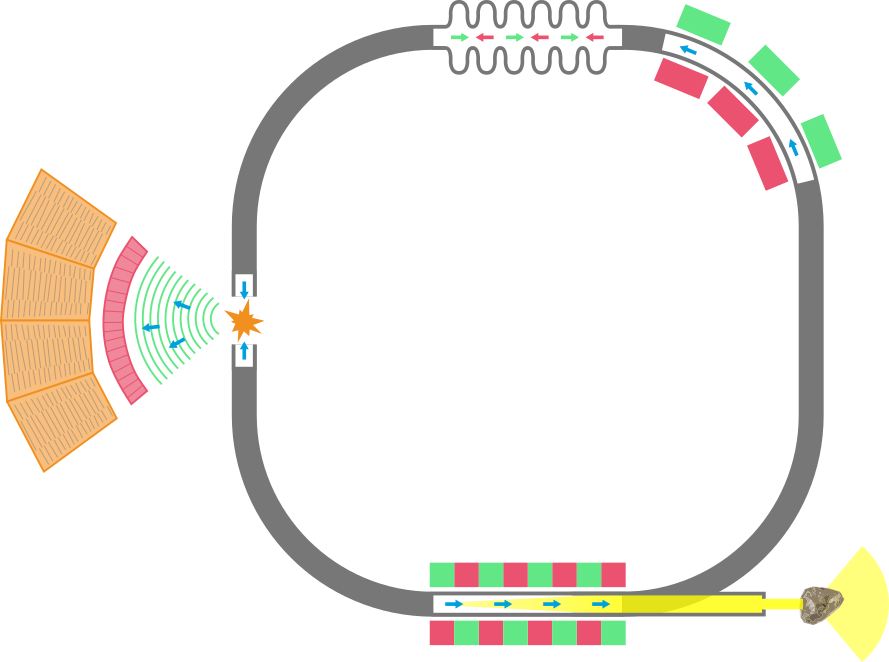
\includegraphics[width=0.9\textwidth]{forschungsgebiete}};
    \node[desyblue] (center) at (1cm,0) {\Large\textbf{Beschleuniger}};
    \node[desyblue,above=0.8cm of center] {\Large\textbf{Teilchenphysik}};
    \node[desyblue,below=0.8cm of center] {\Large\textbf{Forschung mit Photonen}};
\end{tikzpicture}
\vspace*{-11pt}
\end{frame}


\subsection{Beschleuniger}

\begin{frame}
\frametitle{Beschleuniger}
\vspace*{-2\baselineskip}
\begin{tikzpicture}
    \node[inner sep=0pt] at (0,0) {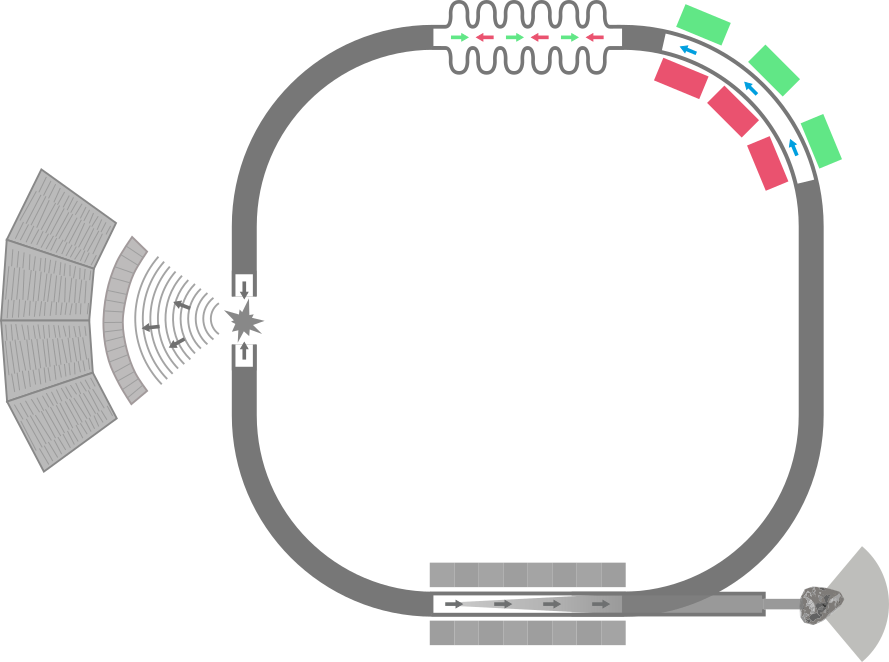
\includegraphics[width=0.9\textwidth]{forschungsgebiete-beschleuniger}};
    \begin{scope}
        \clip [rounded corners=1.5cm] (-1.5cm,-2.4cm) rectangle (3.5cm,2.6cm);
        \node [inner sep=0pt] at (1cm,0.1cm) {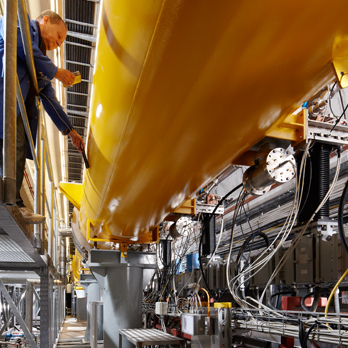
\includegraphics[width=5cm]{gebiet-beschleuniger}};
    \end{scope}
\end{tikzpicture}
\vspace*{-11pt}
\end{frame}


\begin{frame}
\frametitle{Elektrische und magnetische Felder}
\vspace*{-2\baselineskip}
\begin{columns}
\column{0.472\textwidth}\textbf{Elektrische Felder} \\[1em]
\begin{tikzpicture}
    \node [inner sep=0pt] {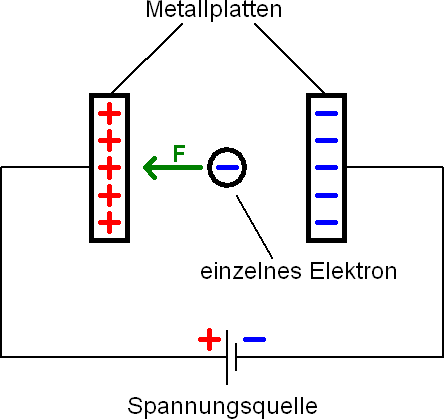
\includegraphics[width=\textwidth]{beschleuniger-efeld}};
    \node [inner sep=2pt,fill=white] at (0cm,2.5cm) {Metallplatten};
    \node [inner sep=2pt,fill=white] at (1cm,-0.8cm) {einzelnes Elektron};
    \node [inner sep=2pt,fill=white] at (0cm,-2.5cm) {Spannungsquelle};
\end{tikzpicture}
\column{0.472\textwidth}\textbf{Magnetische Felder} \\[1ex]
    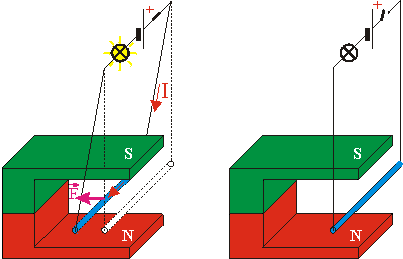
\includegraphics[width=\textwidth]{beschleuniger-lorentzkraft-hufeisen} \\[1em]
    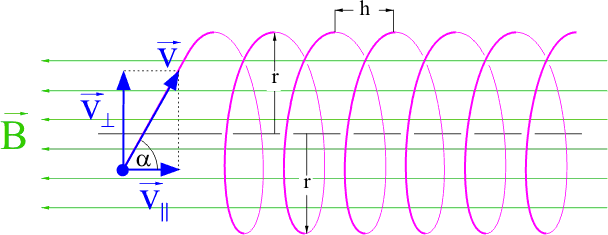
\includegraphics[width=\textwidth]{beschleuniger-lorentzkraft-spirale}
\end{columns}
\vspace*{1em}
\begin{columns}
\column{0.472\textwidth}\centering$\boldsymbol{\Rightarrow}$ \textbf{Beschleunigung}
\column{0.472\textwidth}\centering$\boldsymbol{\Rightarrow}$ \textbf{Ablenkung}
\end{columns}
\end{frame}


\begin{frame}
\frametitle{Was ist ein Teilchenbeschleuniger?}
\vspace*{-2\baselineskip}
\begin{columns}[c]
\column{0.472\textwidth}\begin{itemize}
    \item Ziel: hochenergetische Teilchen
    \begin{itemize}
        \item ``je höher die Energie, desto kleiner die untersuchte Probe''
        \item Energie-Masse-Äquivalenz: $E=mc^2$ (Einstein, 1905)
    \end{itemize}
    \item beschleunigte Teilchen mit der Lorentzkraft: $\vec{F}=q\Big(\vec{E}+\vec{v}\times\vec{B}\Big)$
    \begin{itemize}
        \item Beschleunigung parallel zum elektrischen Feld ($\vec{E}$)
        \item Ablenkung senkrecht zum magnetischen Feld ($\vec{B}$)
    \end{itemize}
    \item erreichte Energien bei HERA:
    \begin{itemize}
        \item Elektronen mit 27.5\,GeV $\approx$~99.999\,999\,98\,\% der Lichtgeschwindigkeit
    \end{itemize}
\end{itemize}
\column{0.472\textwidth}\centering
    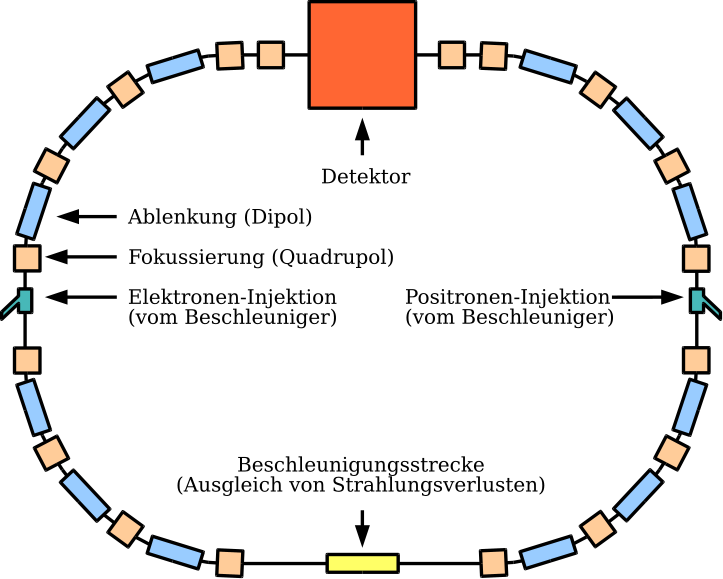
\includegraphics[width=0.8\textwidth]{beschleuniger-schema-de} \\[1em]
    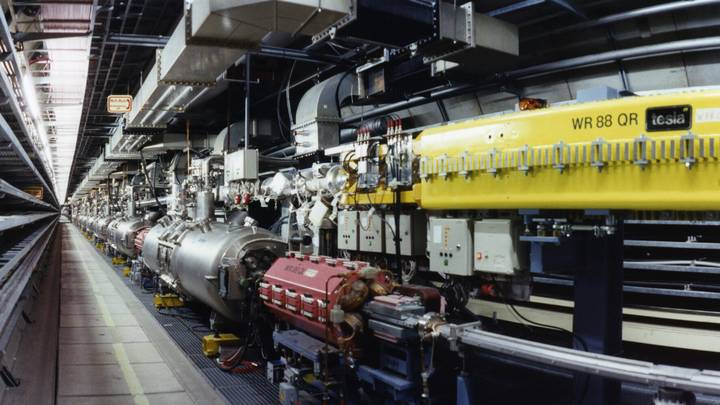
\includegraphics[width=\textwidth,trim={0 0 0 0},clip]{beschleuniger-tunnel}
\end{columns}
\end{frame}

%
% Beschleuniger am DESY
%

\begin{frame}
\frametitle{Beschleuniger: DESY}
\vspace*{-2\baselineskip}
\begin{tikzpicture}[every node/.style={anchor=south east,inner sep=0pt}, x=0mm, y=0mm]   
    \only<1>{\node (photo) at (0,0) {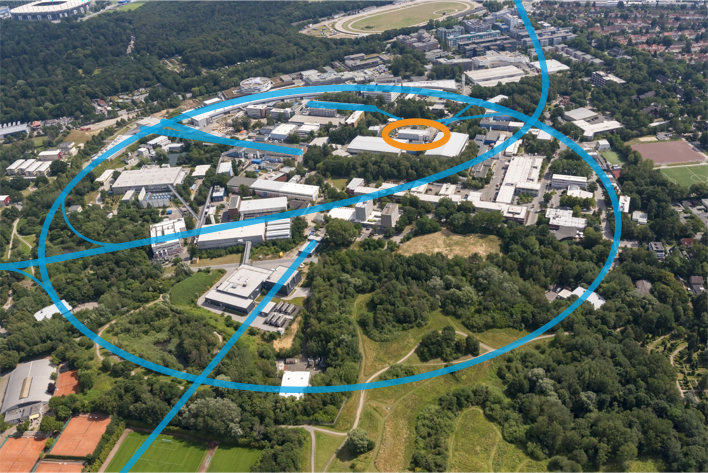
\includegraphics[width=\textwidth]{images/beschleuniger-uebersicht-overlay-desy2.pdf}};}
    \only<2>{\node at (0, 0) {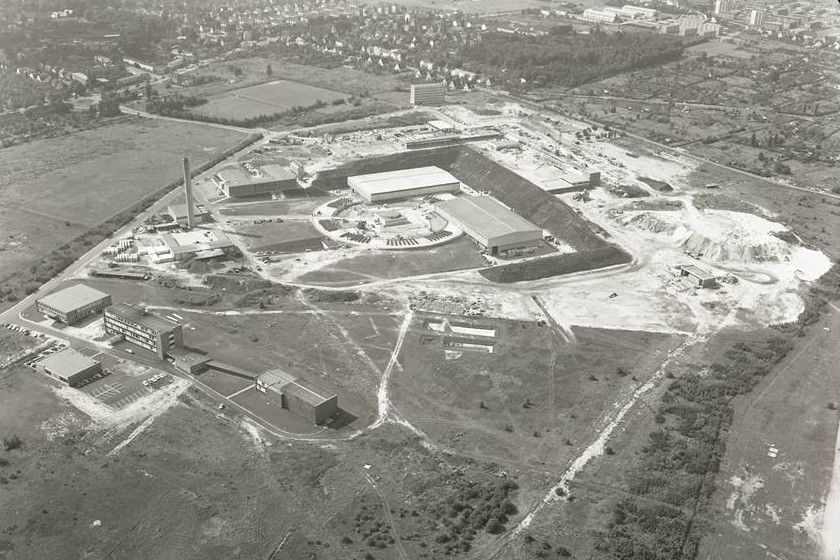
\includegraphics[width=\textwidth]{foto_desy_1963_resized}};}
    \node[inner sep=3pt, rounded corners=3pt, draw, fill=white] (description) at (-0.5cm, 0.5cm) {\parbox{0.45\textwidth}{\raggedright%
        \textbf{D}eutsches \textbf{E}lektronen-\textbf{Sy}nchrotron \\[1ex]
        Erstinbetriebnahme: 1964 \\
        Umfang: 317\,m \\
        Energie: 7,4\,GeV
    }};
\end{tikzpicture}
\end{frame}

\begin{frame}
\frametitle{Beschleuniger: PETRA}
\vspace*{-2\baselineskip}
\begin{tikzpicture}[every node/.style={anchor=south east,inner sep=0pt}, x=0mm, y=0mm]   
    \only<1>{\node at (0,0) {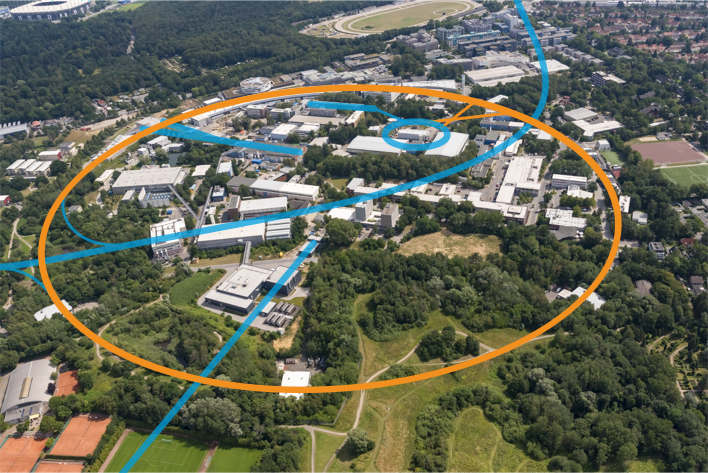
\includegraphics[width=\textwidth]{images/beschleuniger-uebersicht-overlay-petra3.pdf}};}
    \only<2>{\node at (0,0) {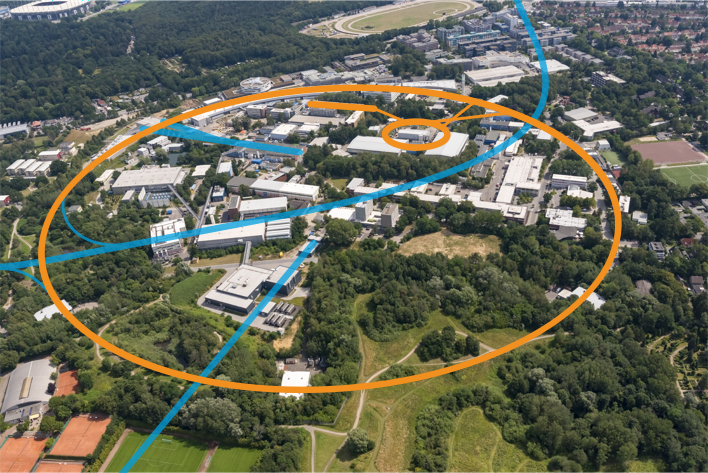
\includegraphics[width=\textwidth]{images/beschleuniger-uebersicht-overlay-petra3-verbund.pdf}};}
    \node[inner sep=3pt, rounded corners=3pt, draw, fill=white] (description) at (-0.5cm, 0.5cm) {%
        \parbox{0.55\textwidth}{\raggedright%
            \textbf{P}ositronen-\textbf{E}lektronen-\textbf{T}andem-\textbf{R}inganlage \\[1ex]
            Erstinbetriebnahme: 1978 \\
            Umfang: 2304\,m \\
            Energie: 19\,GeV (heute 6\,GeV)
        }};
\end{tikzpicture}
\end{frame}

\begin{frame}
\frametitle{Beschleuniger: HERA}
\vspace*{-2\baselineskip}
\begin{tikzpicture}[every node/.style={anchor=south east,inner sep=0pt}, x=0mm, y=0mm]   
    \only<1>{\node (photo) at (0,0) {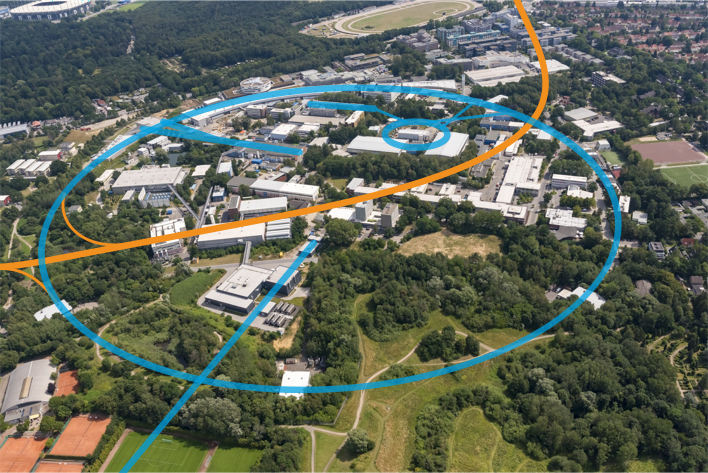
\includegraphics[width=\textwidth]{images/beschleuniger-uebersicht-overlay-hera.pdf}};}
    \only<2>{\node (photo) at (0,0) {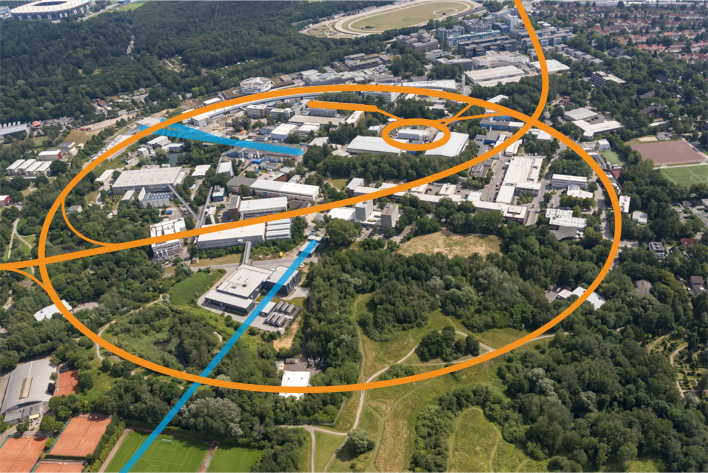
\includegraphics[width=\textwidth]{images/beschleuniger-uebersicht-overlay-hera-verbund.pdf}};}
    \node[inner sep=3pt, rounded corners=3pt, draw, fill=white] (description) at (-0.5cm, 0.5cm) {%
        \parbox{0.50\textwidth}{\raggedright%
            \textbf{H}adronen-\textbf{E}lektronen-\textbf{R}ing-\textbf{A}nlage \\[1ex]
            Erstinbetriebnahme: 1992 \\
            Umfang: 6336\,m \\
            Energie: 27,5\,GeV ($\mathrm{e^-}$/$\mathrm{e^+}$), 980\,GeV ($\mathrm{p^+}$) \\
        }};
\end{tikzpicture}
\end{frame}

\begin{frame}
\frametitle{Beschleuniger: FLASH}
\vspace*{-2\baselineskip}
\begin{tikzpicture}[every node/.style={anchor=south east,inner sep=0pt}, x=0mm, y=0mm]   
    \node (photo) at (0,0) {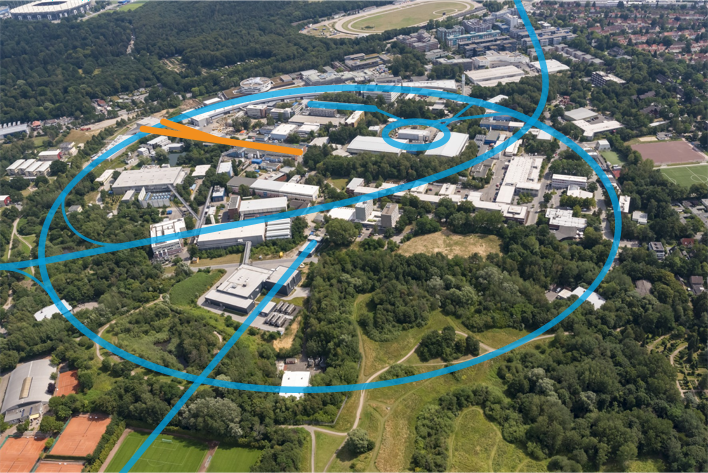
\includegraphics[width=\textwidth]{images/beschleuniger-uebersicht-overlay-flash.pdf}};
    \node[inner sep=3pt, rounded corners=3pt, draw, fill=white] (description) at (-0.5cm, 0.5cm) {%
        \parbox{0.50\textwidth}{\raggedright%
            \textbf{F}reie-Elektronen-\textbf{LAS}er in \textbf{H}amburg \\[1ex]
            Erstinbetriebnahme: 2005 \\
            Länge: 315\,m \\
            Energie: 1,2\,GeV
        }};
\end{tikzpicture}
\end{frame}

\begin{frame}
\frametitle{Beschleuniger: XFEL}
\vspace*{-2\baselineskip}
\begin{tikzpicture}[every node/.style={anchor=south east,inner sep=0pt}, x=0mm, y=0mm]   
    \node (photo) at (0,0) {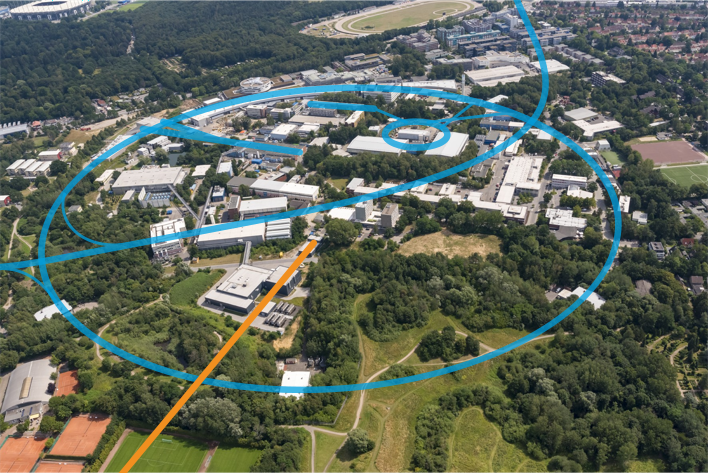
\includegraphics[width=\textwidth]{images/beschleuniger-uebersicht-overlay-xfel.pdf}};
    \only<2>{\node[draw=white, very thick] at (-3mm, 3.6cm) {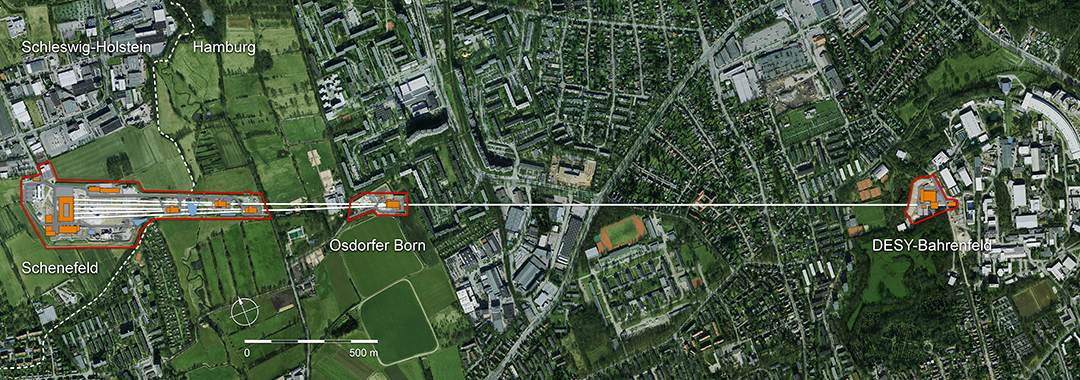
\includegraphics[width=0.95\textwidth]{images/photonen-xfel.jpg}};}
    \node[inner sep=3pt, rounded corners=3pt, draw, fill=white] (description) at (-0.5cm, 0.5cm) {%
        \parbox{0.50\textwidth}{\raggedright%
            \textbf{X}-Ray \textbf{F}reie-\textbf{E}lektronen-\textbf{L}aser \\[1ex]
            Erstinbetriebnahme: 2017 \\
            Länge: 3,4\,km \\
            Energie: 17,5\,GeV
        }};
\end{tikzpicture}
\end{frame}



\subsection{Teilchenphysik}

\begin{frame}
\frametitle{Teilchenphysik}
\vspace*{-2\baselineskip}
\begin{tikzpicture}
    \node[inner sep=0pt] at (0,0) {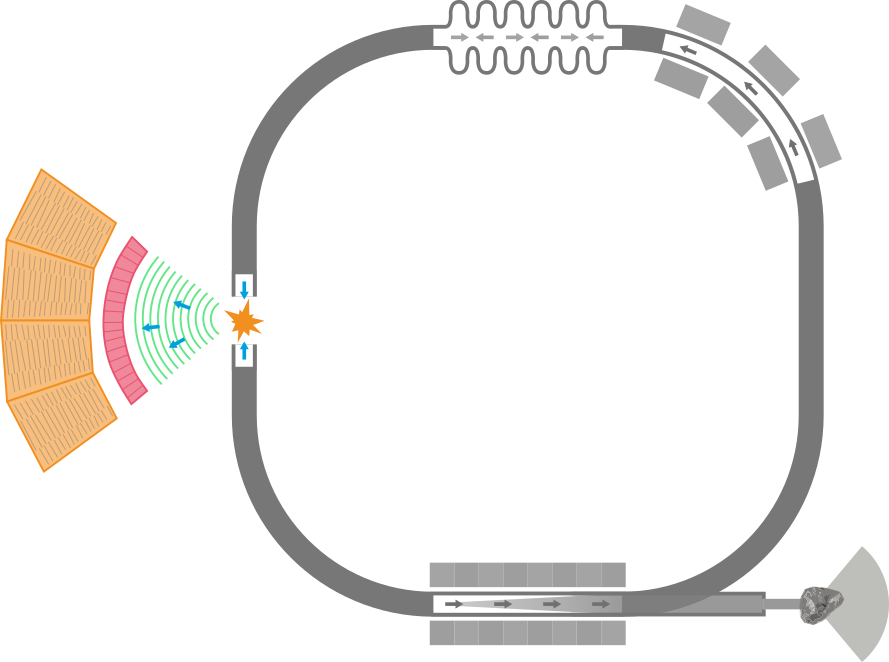
\includegraphics[width=0.9\textwidth]{forschungsgebiete-teilchenphysik}};
    \begin{scope}
        \clip [rounded corners=1.5cm] (-1.5cm,-2.4cm) rectangle (3.5cm,2.6cm);
        \node [inner sep=0pt] at (1cm,0.1cm) {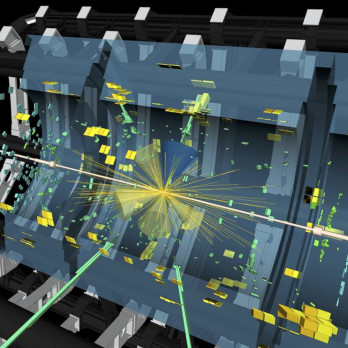
\includegraphics[width=5cm]{gebiet-teilchenphysik}};
    \end{scope}
\end{tikzpicture}
\vspace*{-11pt}
\end{frame}

\begin{frame}
\frametitle{Was ist Teilchenphysik?}
\vspace*{-\baselineskip}\normalsize
\begin{tikzpicture}
    \node [inner sep=0pt] {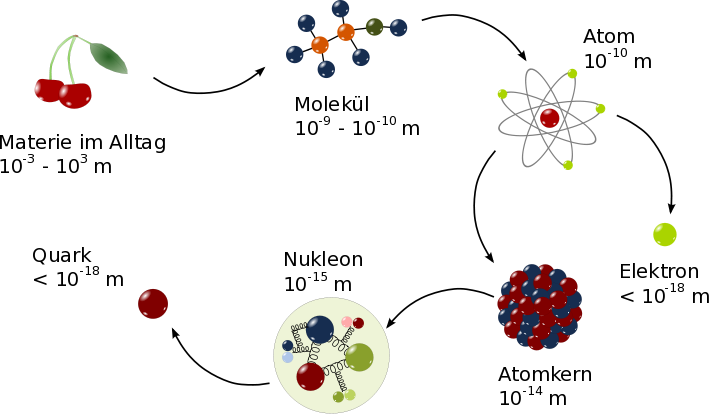
\includegraphics[width=\textwidth]{teilchenphysik-materie}};
\end{tikzpicture}
\end{frame}


\begin{frame}\centering
\frametitle{Standardmodell der Teilchenphysik}
\vspace*{-2.5\baselineskip}
\begin{columns}
\column{0.87\textwidth}~\\[-\baselineskip]
    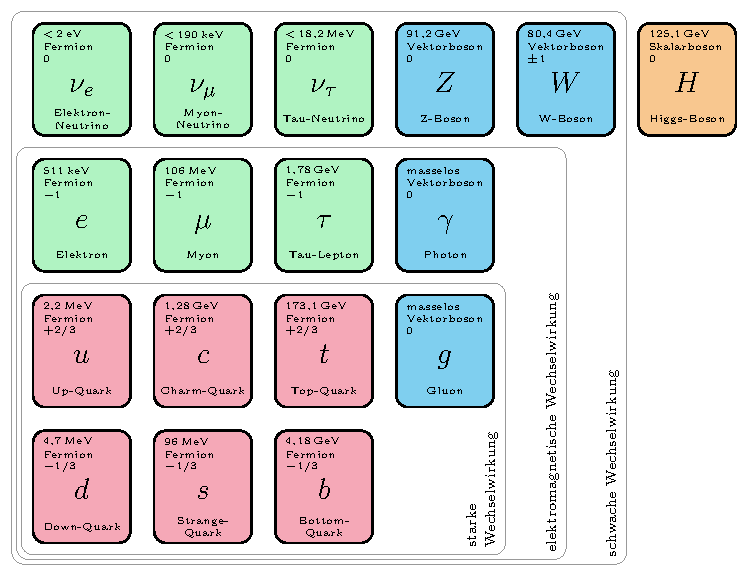
\includegraphics[width=\textwidth]{standardmodell-de}
\column{0.074\textwidth}~\\[4cm]
    \makebox[\textwidth][r]{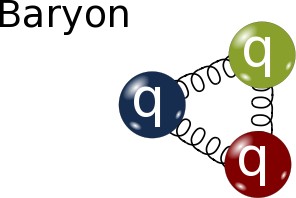
\includegraphics[width=2cm]{teilchenphysik-baryon}} \\[0.5cm]
    \makebox[\textwidth][r]{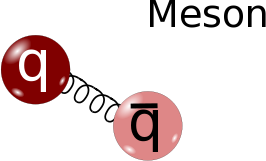
\includegraphics[width=1.8cm]{teilchenphysik-meson}}
\end{columns}
\vspace*{-5pt}
\end{frame}

\begin{frame}
\frametitle{Standardmodell der Teilchenphysik}
\vspace*{-2.0\baselineskip}
\scalebox{0.65}{
    \begin{minipage}{17cm}
        \begin{math}
            -\frac{1}{2}\partial_{\nu}g^{a}_{\mu}\partial_{\nu}g^{a}_{\mu}
            -g_{s}f^{abc}\partial_{\mu}g^{a}_{\nu}g^{b}_{\mu}g^{c}_{\nu}
            -\frac{1}{4}g^{2}_{s}f^{abc}f^{ade}g^{b}_{\mu}g^{c}_{\nu}g^{d}_{\mu}g^{e}_{\nu}
            +\frac{1}{2}ig^{2}_{s}(\bar{q}^{\sigma}_{i}\gamma^{\mu}q^{\sigma}_{j})g^{a}_{\mu}
            +\bar{G}^{a}\partial^{2}G^{a}+g_{s}f^{abc}\partial_{\mu}\bar{G}^{a}G^{b}g^{c}_{\mu}
            -\partial_{\nu}W^{+}_{\mu}\partial_{\nu}W^{-}_{\mu}-M^{2}W^{+}_{\mu}W^{-}_{\mu}
            -\frac{1}{2}\partial_{\nu}Z^{0}_{\mu}\partial_{\nu}Z^{0}_{\mu}-\frac{1}{2c^{2}_{w}}
            M^{2}Z^{0}_{\mu}Z^{0}_{\mu}
            -\frac{1}{2}\partial_{\mu}A_{\nu}\partial_{\mu}A_{\nu}
            -\frac{1}{2}\partial_{\mu}H\partial_{\mu}H-\frac{1}{2}m^{2}_{h}H^{2}
            -\partial_{\mu}\phi^{+}\partial_{\mu}\phi^{-}-M^{2}\phi^{+}\phi^{-}
            -\frac{1}{2}\partial_{\mu}\phi^{0}\partial_{\mu}\phi^{0}-\frac{1}{2c^{2}_{w}}M\phi^{0}\phi^{0}
            -\beta_{h}[\frac{2M^{2}}{g^{2}}+\frac{2M}{g}H+\frac{1}{2}(H^{2}+\phi^{0}\phi^{0}+2\phi^{+}\phi^{-%%@
            })]+\frac{2M^{4}}{g^{2}}\alpha_{h}
            -igc_{w}[\partial_{\nu}Z^{0}_{\mu}(W^{+}_{\mu}W^{-}_{\nu}-W^{+}_{\nu}W^{-}_{\mu})
            -Z^{0}_{\nu}(W^{+}_{\mu}\partial_{\nu}W^{-}_{\mu}-W^{-}_{\mu}\partial_{\nu}W^{+}_{\mu})
            +Z^{0}_{\mu}(W^{+}_{\nu}\partial_{\nu}W^{-}_{\mu}-W^{-}_{\nu}\partial_{\nu}W^{+}_{\mu})]
            -igs_{w}[\partial_{\nu}A_{\mu}(W^{+}_{\mu}W^{-}_{\nu}-W^{+}_{\nu}W^{-}_{\mu})
            -A_{\nu}(W^{+}_{\mu}\partial_{\nu}W^{-}_{\mu}-W^{-}_{\mu}\partial_{\nu}W^{+}_{\mu})
            +A_{\mu}(W^{+}_{\nu}\partial_{\nu}W^{-}_{\mu}-W^{-}_{\nu}\partial_{\nu}W^{+}_{\mu})]
            -\frac{1}{2}g^{2}W^{+}_{\mu}W^{-}_{\mu}W^{+}_{\nu}W^{-}_{\nu}+\frac{1}{2}g^{2}
            W^{+}_{\mu}W^{-}_{\nu}W^{+}_{\mu}W^{-}_{\nu}
            +g^2c^{2}_{w}(Z^{0}_{\mu}W^{+}_{\mu}Z^{0}_{\nu}W^{-}_{\nu}-Z^{0}_{\mu}Z^{0}_{\mu}W^{+}_{\nu}
            W^{-}_{\nu})
            +g^2s^{2}_{w}(A_{\mu}W^{+}_{\mu}A_{\nu}W^{-}_{\nu}-A_{\mu}A_{\mu}W^{+}_{\nu}
            W^{-}_{\nu})
            +g^{2}s_{w}c_{w}[A_{\mu}Z^{0}_{\nu}(W^{+}_{\mu}W^{-}_{\nu}-W^{+}_{\nu}W^{-}_{\mu})-%%@
            2A_{\mu}Z^{0}_{\mu}W^{+}_{\nu}W^{-}_{\nu}]
            -g\alpha[H^3+H\phi^{0}\phi^{0}+2H\phi^{+}\phi^{-}]
            -\frac{1}{8}g^{2}\alpha_{h}[H^4+(\phi^{0})^{4}+4(\phi^{+}\phi^{-})^{2}+4(\phi^{0})^{2}
            \phi^{+}\phi^{-}+4H^{2}\phi^{+}\phi^{-}+2(\phi^{0})^{2}H^{2}]
            -gMW^{+}_{\mu}W^{-}_{\mu}H-\frac{1}{2}g\frac{M}{c^{2}_{w}}Z^{0}_{\mu}Z^{0}_{\mu}H
            -\frac{1}{2}ig[W^{+}_{\mu}(\phi^{0}\partial_{\mu}\phi^{-}-\phi^{-}\partial_{\mu}\phi^{0})
            -W^{-}_{\mu}(\phi^{0}\partial_{\mu}\phi^{+}-\phi^{+}\partial_{\mu}\phi^{0})]
            +\frac{1}{2}g[W^{+}_{\mu}(H\partial_{\mu}\phi^{-}-\phi^{-}\partial_{\mu}H)
            -W^{-}_{\mu}(H\partial_{\mu}\phi^{+}-\phi^{+}\partial_{\mu}H)]
            +\frac{1}{2}g\frac{1}{c_{w}}(Z^{0}_{\mu}(H\partial_{\mu}\phi^{0}-\phi^{0}\partial_{\mu}H)
            -ig\frac{s^{2}_{w}}{c_{w}}MZ^{0}_{\mu}(W^{+}_{\mu}\phi^{-}-W^{-}_{\mu}\phi^{+})
            +igs_{w}MA_{\mu}(W^{+}_{\mu}\phi^{-}-W^{-}_{\mu}\phi^{+})
            -ig\frac{1-2c^{2}_{w}}{2c_{w}}Z^{0}_{\mu}(\phi^{+}\partial_{\mu}\phi^{-}-\phi^{-%%@
            }\partial_{\mu}\phi^{+})
            +igs_{w}A_{\mu}(\phi^{+}\partial_{\mu}\phi^{-}-\phi^{-}\partial_{\mu}\phi^{+})
            -\frac{1}{4}g^{2}W^{+}_{\mu}W^{-}_{\mu}[H^{2}+(\phi^{0})^{2}+2\phi^{+}\phi^{-}]
            -\frac{1}{4}g^{2}\frac{1}{c^{2}_{w}}Z^{0}_{\mu}Z^{0}_{\mu}[H^{2}+(\phi^{0})^{2}+2(2s^{2}_{w}-%%@
            1)^{2}\phi^{+}\phi^{-}]
            -\frac{1}{2}g^{2}\frac{s^{2}_{w}}{c_{w}}Z^{0}_{\mu}\phi^{0}(W^{+}_{\mu}\phi^{-}+W^{-%%@
            }_{\mu}\phi^{+})
            -\frac{1}{2}ig^{2}\frac{s^{2}_{w}}{c_{w}}Z^{0}_{\mu}H(W^{+}_{\mu}\phi^{-}-W^{-}_{\mu}\phi^{+})
            +\frac{1}{2}g^{2}s_{w}A_{\mu}\phi^{0}(W^{+}_{\mu}\phi^{-}+W^{-}_{\mu}\phi^{+})
            +\frac{1}{2}ig^{2}s_{w}A_{\mu}H(W^{+}_{\mu}\phi^{-}-W^{-}_{\mu}\phi^{+})
            -g^{2}\frac{s_{w}}{c_{w}}(2c^{2}_{w}-1)Z^{0}_{\mu}A_{\mu}\phi^{+}\phi^{-}-%%@
            g^{1}s^{2}_{w}A_{\mu}A_{\mu}\phi^{+}\phi^{-}
            -\bar{e}^{\lambda}(\gamma\partial+m^{\lambda}_{e})e^{\lambda}
            -\bar{\nu}^{\lambda}\gamma\partial\nu^{\lambda}
            -\bar{u}^{\lambda}_{j}(\gamma\partial+m^{\lambda}_{u})u^{\lambda}_{j}
            -\bar{d}^{\lambda}_{j}(\gamma\partial+m^{\lambda}_{d})d^{\lambda}_{j}
            +igs_{w}A_{\mu}[-(\bar{e}^{\lambda}\gamma^{\mu}
            e^{\lambda})+\frac{2}{3}(\bar{u}^{\lambda}_{j}\gamma^{\mu} %%@
            u^{\lambda}_{j})-\frac{1}{3}(\bar{d}^{\lambda}_{j}\gamma^{\mu} 
            d^{\lambda}_{j})]
            +\frac{ig}{4c_{w}}Z^{0}_{\mu}
            [(\bar{\nu}^{\lambda}\gamma^{\mu}(1+\gamma^{5})\nu^{\lambda})+
            (\bar{e}^{\lambda}\gamma^{\mu}(4s^{2}_{w}-1-\gamma^{5})e^{\lambda})+
            (\bar{u}^{\lambda}_{j}\gamma^{\mu}(\frac{4}{3}s^{2}_{w}-1-\gamma^{5})u^{\lambda}_{j})+
            (\bar{d}^{\lambda}_{j}\gamma^{\mu}(1-\frac{8}{3}s^{2}_{w}-\gamma^{5})d^{\lambda}_{j})]
            +\frac{ig}{2\sqrt{2}}W^{+}_{\mu}[(\bar{\nu}^{\lambda}\gamma^{\mu}(1+\gamma^{5})e^{\lambda})
            +(\bar{u}^{\lambda}_{j}\gamma^{\mu}(1+\gamma^{5})C_{\lambda\kappa}d^{\kappa}_{j})]
            +\frac{ig}{2\sqrt{2}}W^{-}_{\mu}[(\bar{e}^{\lambda}\gamma^{\mu}(1+\gamma^{5})\nu^{\lambda})
            +(\bar{d}^{\kappa}_{j}C^{\dagger}_{\lambda\kappa}\gamma^{\mu}(1+\gamma^{5})u^{\lambda}_{j})]
            +\frac{ig}{2\sqrt{2}}\frac{m^{\lambda}_{e}}{M}
            [-\phi^{+}(\bar{\nu}^{\lambda}(1-\gamma^{5})e^{\lambda})
            +\phi^{-}(\bar{e}^{\lambda}(1+\gamma^{5})\nu^{\lambda})]
            -\frac{g}{2}\frac{m^{\lambda}_{e}}{M}[H(\bar{e}^{\lambda}e^{\lambda})
            +i\phi^{0}(\bar{e}^{\lambda}\gamma^{5}e^{\lambda})]
            +\frac{ig}{2M\sqrt{2}}\phi^{+}
            [-m^{\kappa}_{d}(\bar{u}^{\lambda}_{j}C_{\lambda\kappa}(1-\gamma^{5})d^{\kappa}_{j})
            +m^{\lambda}_{u}(\bar{u}^{\lambda}_{j}C_{\lambda\kappa}(1+\gamma^{5})d^{\kappa}_{j}]
            +\frac{ig}{2M\sqrt{2}}\phi^{-}
            [m^{\lambda}_{d}(\bar{d}^{\lambda}_{j}C^{\dagger}_{\lambda\kappa}(1+\gamma^{5})u^{\kappa}_{j})
            -m^{\kappa}_{u}(\bar{d}^{\lambda}_{j}C^{\dagger}_{\lambda\kappa}(1-\gamma^{5})u^{\kappa}_{j}]
            -\frac{g}{2}\frac{m^{\lambda}_{u}}{M}H(\bar{u}^{\lambda}_{j}u^{\lambda}_{j})
            -\frac{g}{2}\frac{m^{\lambda}_{d}}{M}H(\bar{d}^{\lambda}_{j}d^{\lambda}_{j})
            +\frac{ig}{2}\frac{m^{\lambda}_{u}}{M}\phi^{0}(\bar{u}^{\lambda}_{j}\gamma^{5}u^{\lambda}_{j})
            -\frac{ig}{2}\frac{m^{\lambda}_{d}}{M}\phi^{0}(\bar{d}^{\lambda}_{j}\gamma^{5}d^{\lambda}_{j})
            +\bar{X}^{+}(\partial^{2}-M^{2})X^{+}+\bar{X}^{-}(\partial^{2}-M^{2})X^{-}
            +\bar{X}^{0}(\partial^{2}-\frac{M^{2}}{c^{2}_{w}})X^{0}+\bar{Y}\partial^{2}Y
            +igc_{w}W^{+}_{\mu}(\partial_{\mu}\bar{X}^{0}X^{-}-\partial_{\mu}\bar{X}^{+}X^{0})
            +igs_{w}W^{+}_{\mu}(\partial_{\mu}\bar{Y}X^{-}-\partial_{\mu}\bar{X}^{+}Y)
            +igc_{w}W^{-}_{\mu}(\partial_{\mu}\bar{X}^{-}X^{0}-\partial_{\mu}\bar{X}^{0}X^{+})
            +igs_{w}W^{-}_{\mu}(\partial_{\mu}\bar{X}^{-}Y-\partial_{\mu}\bar{Y}X^{+})
            +igc_{w}Z^{0}_{\mu}(\partial_{\mu}\bar{X}^{+}X^{+}-\partial_{\mu}\bar{X}^{-}X^{-})
            +igs_{w}A_{\mu}(\partial_{\mu}\bar{X}^{+}X^{+}-\partial_{\mu}\bar{X}^{-}X^{-})
            -\frac{1}{2}gM[\bar{X}^{+}X^{+}H+\bar{X}^{-}X^{-}H+\frac{1}{c^{2}_{w}}\bar{X}^{0}X^{0}H]
            +\frac{1-2c^{2}_{w}}{2c_{w}}igM[\bar{X}^{+}X^{0}\phi^{+}-\bar{X}^{-}X^{0}\phi^{-}]
            +\frac{1}{2c_{w}}igM[\bar{X}^{0}X^{-}\phi^{+}-\bar{X}^{0}X^{+}\phi^{-}]
            +igMs_{w}[\bar{X}^{0}X^{-}\phi^{+}-\bar{X}^{0}X^{+}\phi^{-}]
            +\frac{1}{2}igM[\bar{X}^{+}X^{+}\phi^{0}-\bar{X}^{-}X^{-}\phi^{0}]
        \end{math}
        \\[2ex]
        Extrahiert von Thomas\,D.\,Gutierrez aus Diagrammatica von Martinus Veltman irgendwann 1999.\cite{web:stml}
    \end{minipage}
}
\end{frame}


\begin{frame}
\frametitle{Kollisions-Experiment}
\vspace*{-2\baselineskip}
\begin{columns}
\column{0.151\textwidth}\textbf{Verfügbar:}
\column{0.793\textwidth}Stabile Teilchen \\
    \qquad\textbullet~~ Elektronen \\
    \qquad\textbullet~~ Protonen (zusammengesetzt aus Quarks)
\end{columns}
\vspace*{1ex}
\begin{columns}
\column{0.151\textwidth}\textbf{Gesucht:}
\column{0.793\textwidth}seltene Teilchen, z.B. Higgs-Boson, Top-Quark, B-Meson \\
    \qquad$\Rightarrow$~~ instabil, zerfallen schnell zu vielen leichteren Teilchen \\
    \qquad$\Rightarrow$~~ sehr hohe Masse, d.h. viel Energie zur Erzeugung nötig
\end{columns}
\vspace*{1ex}
\begin{columns}
\column{0.151\textwidth}\textbf{Experiment:}
\column{0.793\textwidth}1. Kollision von zwei hochenergetischen Teilchen \\
    \qquad$\Rightarrow$~~ schwere Teilchen können erzeugt werden \\[1ex]
    2. Messung der Zerfallsprodukte mit großen Detektoren \\
    \qquad$\Rightarrow$~~ Rekonstruktion der schweren Teilchen \\
    \qquad$\Rightarrow$~~ statistische Analyse
\end{columns}
\vspace*{1ex}
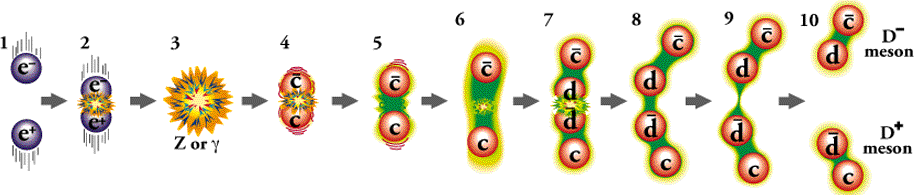
\includegraphics[width=\textwidth]{teilchenphysik-kollision}
\end{frame}


\begin{frame}
\frametitle{Beispiel: CMS Experiment at the LHC}
\vspace*{-2.5\baselineskip}
Das \textbf{C}ompact-\textbf{M}uon-\textbf{S}olenoid-Experiment ist eines von vier Experimenten am \textbf{L}arge \textbf{H}adron \textbf{C}ollider, dem größten Teilchenbeschleuniger der Welt, am CERN. \\[\baselineskip]
\makebox[\textwidth]{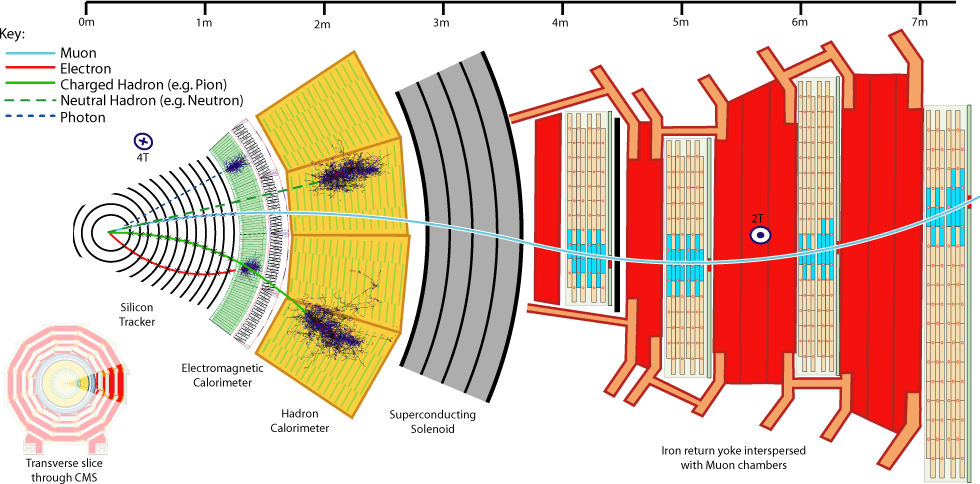
\includegraphics[width=0.99\paperwidth]{teilchenphysik-detektor}}
\vspace*{-18pt}
\end{frame}


\begin{frame}
\frametitle{Entdeckung des Gluons bei PETRA}
\vspace*{-2.6\baselineskip}
\alert{\bfseries\footnotesize R. Brandelik et al. (TASSO Collaboration), Evidence for planar events in e\textsuperscript{+}e\textsuperscript{--} annihilation at high energies, Physics Letters 86B, 243--249 (1979) \cite{Brandelik1979}}
\vspace*{\baselineskip}
\begin{columns}
\column{0.2\textwidth}
    \textbf{nur Quarks} \\
    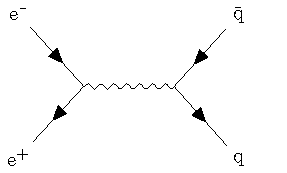
\includegraphics[width=\textwidth,page=1]{gluon-feynman} \\[1ex]
    \textbf{mit Gluonen} \\
    \includegraphics[width=\textwidth,page=2]{gluon-feynman} \\
    \includegraphics[width=\textwidth,page=3]{gluon-feynman} \\
    \includegraphics[width=\textwidth,page=4]{gluon-feynman}
\column{0.744\textwidth}Die Experimente bei PETRA beobachteten Ereignisse mit drei Jets. Diese konnten nicht allein mit Quarks erklärt werden \\
$\Rightarrow$ die Gluonen waren entdeckt \\[1ex]
    \centering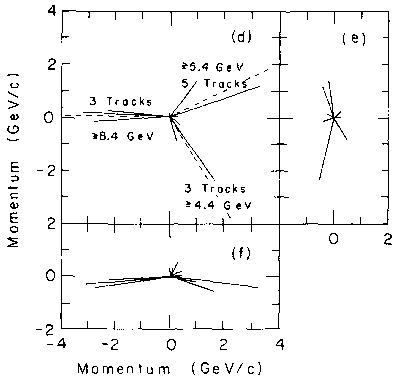
\includegraphics[width=0.7\textwidth]{gluon-threejets}
\end{columns}
\vspace*{-18pt}
\end{frame}


\begin{frame}
\frametitle{Struktur des Protons bei HERA}
\vspace*{-2.6\baselineskip}
\alert{\bfseries\footnotesize H. Abramowicz et al. (H1 and ZEUS Collaborations), Combination of measurements of inclusive deep inelastic e\textsuperscript{$\pm$}p scattering cross sections and QCD analysis of HERA data, European Physical Journal C75 (2015) 12, 580 \cite{Abramowicz2015}}
\vspace*{\baselineskip}
\begin{columns}
\column{0.472\textwidth}~\\[-\baselineskip]
\begin{minipage}[c]{0.3\textwidth}
    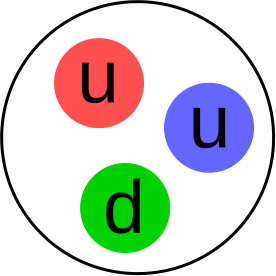
\includegraphics[width=\textwidth]{hera-proton1}
\end{minipage}
\hfill
\begin{minipage}[c]{0.65\textwidth}\raggedright
    Das Proton besteht aus drei ``Valenzquarks'', zwei Up- und ein Down-Quark
\end{minipage}\vspace*{1ex}

Diese Quarks interagieren aber ständig über die starke Wechselwirkung, sodass auch Gluonen, andere Quarks und Anti-Quarks im Proton gefunden werden können.  

\begin{minipage}[c]{0.35\textwidth}
    \includegraphics[width=\textwidth]{hera-proton2}
\end{minipage}
\hfill
\begin{minipage}[c]{0.6\textwidth}\raggedright
Bei HERA konnte die Zusammensetzung des Protons so genau ver- messen werden, dass diese Ergebnisse noch lange führend sein werden.
\end{minipage}
\column{0.472\textwidth}~\\[-\baselineskip]
    \includegraphics[width=\textwidth,trim={2.4cm 1.7cm 1.1cm 0.4cm},clip]{hera-pdf}
\end{columns}
\vspace*{-7pt}
\end{frame}


\begin{frame}
\frametitle{Messung von $\boldsymbol{H\rightarrow b\bar{b}}$ am LHC}
\vspace*{-2.6\baselineskip}
\alert{\bfseries\footnotesize M. Aaboud et al. (ATLAS Collaboration), Observation of $\boldsymbol{H\rightarrow b\bar{b}}$ decays and $\boldsymbol{VH}$ production with the ATLAS detector, Physics Letters B786 (2018) 59--86 \cite{Aaboud2018}}
\vspace*{\baselineskip}
\begin{columns}
\column{0.472\textwidth}\centering~\\[-\baselineskip]
    \includegraphics[width=\textwidth]{vhbb-feynman} \\[1ex]
    \includegraphics[width=0.8\textwidth]{vhbb-lhc}%
    \Put(-15,53){\includegraphics[width=0.6cm]{logos/cms}}%
    \Put(-23,15){\setlength\fboxsep{0pt}\fbox{\includegraphics[height=0.5cm]{vhbb-atlas}}}
\column{0.472\textwidth}~\\[-\baselineskip]
    \includegraphics[width=\textwidth]{vhbb-result} \\[1ex]
    $H\rightarrow b\bar{b}$ kann nur durch statistische Auswertung von $Z\rightarrow b\bar{b}$ unterschieden werden.
\end{columns}
\vspace*{-3pt}
\end{frame}


\begin{frame}
\frametitle{Kosmische Neutrinos mit IceCube}
\vspace*{-2.6\baselineskip}
\alert{\bfseries\footnotesize M. Aartsen et al. (IceCube Collaboration), Neutrino emission from the direction of the blazar TXS 0506+056 prior to the IceCube-170922A alert, Science 361 (2018) 6398 \cite{IceCube}}
\vspace*{\baselineskip}
\begin{columns}
\column{0.472\textwidth}\textbf{Experiment} \\[1ex]
    \includegraphics[width=\textwidth]{icecube-experiment} \\
    Neutrino-Observatorium am Südpol, mit 5160 Sensoren in einem Eisblock von einem Kubikkilometer Größe
\column{0.472\textwidth}\textbf{Ergebnis} \\[1ex]
    \includegraphics[width=\textwidth]{icecube-ergebnis} \\
    Erste Beobachtung eines hochenergetischen Neutrinos (300\,TeV) $\Rightarrow$ weitere Beobachtungen bestätigen die Quelle als Blasar in 4\,Milliarden Lichtjahren Entfernung.
\end{columns}
\vspace*{-8pt}
\end{frame}

\subsection{Forschung mit Photonen}

\begin{frame}
\frametitle{Forschung mit Photonen}
\vspace*{-2\baselineskip}
\begin{tikzpicture}
    \node[inner sep=0pt] at (0,0) {\includegraphics[width=0.9\textwidth]{forschungsgebiete-forschungmitphotonen}};
    \begin{scope}
        \clip [rounded corners=1.5cm] (-1.5cm,-2.4cm) rectangle (3.5cm,2.6cm);
        \node [inner sep=0pt] at (1cm,0.1cm) {\includegraphics[width=5cm]{gebiet-forschungmitphotonen}};
    \end{scope}
\end{tikzpicture}
\vspace*{-11pt}
\end{frame}


\begin{frame}
\frametitle{Beschleuniger als Lichtquellen}
\vspace*{-2.2\baselineskip}
\begin{columns}
\column{0.562\textwidth}~\\[-\baselineskip]
\makebox[\textwidth][l]{\begin{tikzpicture}
    \node [inner sep=0pt] at (0,0) {\includegraphics[width=1.4\textwidth]{photonen-erzeugung}};
\end{tikzpicture}}
\column{0.382\textwidth}~\\ Geladene Teilchen, die auf einer Kreisbahn abgelenkt werden, strahlen Licht ab
\begin{itemize}
    \item ``Synchrotron-Strahlung''
    \item sehr intensives und stark gebündeltes Licht
\end{itemize}
\end{columns}
\vspace*{-7pt}
\end{frame}


\begin{frame}
\frametitle{Experimente mit Licht}
\vspace*{-1.5\baselineskip}
\begin{tikzpicture}
    \node [inner sep=0pt] {\includegraphics[width=\textwidth]{photonen-experiment}};
    \node [shape=circle,draw,fill=white,inner sep=2pt] at (-4cm,2.5cm) {1};
    \node [shape=circle,draw,fill=white,inner sep=2pt] at (-2.17cm,2.5cm) {2};
    \node [shape=circle,draw,fill=white,inner sep=2pt] at (0.8cm,2.5cm) {3};
    \node [shape=circle,draw,fill=white,inner sep=2pt] at (4.7cm,-1.7cm) {4};
    \node [inner sep=0pt] at (-3cm,-2.5cm) {\parbox{5.5cm}{\raggedright\begin{enumerate}
        \item Der Elektronenstrahl erzeugt Licht in magnetischen Strukturen
        \item Die Probe wird bestrahlt
        \item Gestreutes, emittiertes oder nicht absorbiertes Licht wird gemessen
        \item die Struktur der Probe wird aus den gemessenen Daten rekonstruiert
    \end{enumerate}}};
    \node [inner sep=0pt] at (3.8cm,1.2cm) {\parbox{4cm}{\raggedright%
        \textbf{Spektroskopie} bestimmt chemische Vorgänge aus Emissions- und Absorptionsspektren. \\[1ex]
        \textbf{Streuung} bestimmt atomare Strukturen aus Lichtbeugung an Kristallen. \\[1ex]
        \textbf{Bildgebung} stellt Strukturen wie in einem Lichtmikroskop dar.
    }};
\end{tikzpicture}
\vspace*{-22pt}
\end{frame}


\begin{frame}
\frametitle{PETRA III \color{desyorange}\large -- brillianteste Lichtquelle ihrer Art}
\vspace*{-2.5\baselineskip}
\begin{tikzpicture}[every node/.style={anchor=south east,inner sep=0pt}, x=0mm, y=0mm]   
    \node at (0,0) {\includegraphics[width=\textwidth]{photonen-petra3}};
    \node [inner sep=3pt, rounded corners=3pt, draw, fill=white] at (-3mm,3mm) {
        \scalebox{0.5}{\parbox{9cm}{%
            Energie der Elektronen: 6\,GeV \\
            Energie der Photonen: 150\,eV\,--\,200\,keV \\
            Wellenlänge der Photonen: 8\,nm\,--\,0,006\,nm \\
            maximale Brillianz: $1\times10^{21}\,Photons\,/\,(s\,mm^2\,mrad^2\,0.1\,\%\,BW)$
    }}};
\end{tikzpicture}
\vspace*{-4pt}
\end{frame}


\begin{frame}
\frametitle{FLASH \color{desyorange}\large -- weltweit erster FEL für weiches Röntgenlicht}
\vspace*{-2.5\baselineskip}
\begin{tikzpicture}[every node/.style={anchor=south east,inner sep=0pt}, x=0mm, y=0mm]   
    \node at (0,0) {\includegraphics[width=\textwidth]{photonen-flash}};
    \node [inner sep=3pt, rounded corners=3pt, draw, fill=white] at (-3mm, 3mm) {
        \scalebox{0.5}{\parbox{9cm}{%
            Energie der Elektronen: 0,35\,GeV\,--\,1,25\,GeV \\
            Energie der Photonen: 14\,eV\,--\,310\,eV \\
            Wellenlänge der Photonen: 90\,nm\,--\,4\,nm \\
            Pulsdauer: 30\,fs\,--\,200\,fs \\
            maximale Brillianz: $1\times10^{31}\,Photons\,/\,(s\,mm^2\,mrad^2\,0.1\,\%\,BW)$
    }}};
\end{tikzpicture}
\vspace*{-22pt}
\end{frame}


\begin{frame}
\frametitle{European XFEL \color{desyorange}\large -- größter Röntgenlaser der Welt}
\vspace*{-2.5\baselineskip}
\begin{tikzpicture}[every node/.style={anchor=south east,inner sep=0pt}, x=0mm, y=0mm]
    \node at (0,0) {\includegraphics[width=\textwidth]{images/2018-11-22_X-ray-laser-beam_000471.jpg}};
    \node [inner sep=3pt, rounded corners=3pt, draw, fill=white] at (-3mm, 3mm) {
        \scalebox{0.5}{\parbox{9cm}{%
            Energie der Elektronen: bis zu 17,5\,GeV \\
            Energie der Photonen: 0,2\,keV\,--\,25\,keV  \\
            Wellenlänge der Photonen: 4,7\,nm\,--\,0,05\,nm \\
            Pulsdauer: <100\,fs \\
            maximale Brillianz: $5\times10^{33}\,Photons\,/\,(s\,mm^2\,mrad^2\,0.1\,\%\,BW)$
    }}};
\end{tikzpicture}
\end{frame}


\begin{frame}
\frametitle{``FLASH, what a picture!''}
\vspace*{-2.6\baselineskip}
\alert{\bfseries\footnotesize H. Chapman et al., Femtosecond diffractive imaging with a soft-X-ray free-electron laser, Nature Physics 2, 839--843 (2006) \cite{Chapman2006}}
\vspace*{\baselineskip}
\begin{columns}[c]
\column{0.472\textwidth}\includegraphics[width=\textwidth]{flash-aufbau}
\column{0.472\textwidth}\begin{itemize}
    \item Probe mit \textmu m-Struktur beleuchtet mit einzelnem Röntgen-Laserpuls
    \item Beugungsmuster aufgenommen mit CCD-Sensoren (unter veschiedenen Winkeln durch Benutzung eines Spiegelsystems)
\end{itemize}
\end{columns}
\vspace*{1ex}
\begin{columns}[c]
\column{0.25\textwidth}\includegraphics[width=\textwidth]{flash-beugungsbild}
\column{0.3\textwidth}\begin{itemize}
    \item links: aufgenommenes Beugungsbild
    \item rechts: rekonstruiertes Röntgenbild
    \item erste Demonstration hochauflösender Bildgebung mit FLASH
\end{itemize}
\column{0.35\textwidth}\includegraphics[width=\textwidth]{flash-rekonstruiert}
\end{columns}
\vspace*{-3pt}
\end{frame}


\begin{frame}
\frametitle{Biochemie: Ribosomenstruktur}
\vspace*{-2.6\baselineskip}
\alert{\bfseries\footnotesize A. Tocilj et al., The small ribosomal subunit from \textit{Thermus thermophilus} at 4.5\,\AA{} resolution: Pattern fittings and the identification of a functional site, Proc. Natl. Acad. Sci. USA 95 (1999) 25, 14252--14257 \cite{Tocilj1999}}
\vspace*{\baselineskip}
\begin{columns}
\column{0.492\textwidth}~\\[-\baselineskip]
    \includegraphics[width=\textwidth]{ribosom-struktur}
    \vspace*{-1ex}

    \begin{minipage}[c]{0.2\textwidth}
        \includegraphics[width=\textwidth]{nobelpreis}
    \end{minipage}
    \hfill
    \begin{minipage}[c]{0.75\textwidth}\raggedright\footnotesize
        Nobelpreis in Chemie 2009 an Ada Yonath ``für die Studien zur Struktur und Funktion des Ribosoms''
    \end{minipage}
\column{0.452\textwidth}~\\[-\baselineskip]
    \includegraphics[width=\textwidth]{ribosomen-messung}
\end{columns}
\vspace*{-7pt}
\end{frame}


\begin{frame}
\frametitle{Nanopartikel: Katalysator-Oberfläche}
\vspace*{-2.6\baselineskip}
\alert{\bfseries\footnotesize U. Hejral et al., Identification of a catalytically highly active surface phase for CO oxidation over PtRh nanoparticles under operando reaction conditions, Physical Review Letters 120, 126101 (2018) \cite{Hejral2018}}
\vspace*{\baselineskip}
\begin{columns}
    \column{0.532\textwidth}
        ~\\[-\baselineskip]
        \includegraphics[width=\textwidth]{nano-methode}
    \column{0.412\textwidth}
        Untersuchungen zur Reaktivität der Oxidation von
        CO\,$\rightarrow$\,CO\textsubscript{2} an Oberflächen mit Nanopartikeln
        aus Pt-Rh-Legierung zeigt, dass die Reaktivität steigt, wenn der
        Katalysator mehr Ecken hat.
        \vspace*{1ex}
        \includegraphics[width=\textwidth]{nano-3d}
\end{columns}
\end{frame}


\begin{frame}
\frametitle{Kunst: Verborgene Gemälde}
\vspace*{-2.6\baselineskip}
\alert{\bfseries\footnotesize J. Dik et al., Visualization of a lost painting by Vincent van Gogh using synchrotron radiation based X-ray fluorescence elemental mapping, Anal. Chem. 80 (2008) 16 \cite{Dik2008}}
\vspace*{0.5\baselineskip}
\begin{columns}
\column{0.472\textwidth}\textbf{Original: \glqq Grasgrond\grqq\\(Vincent van Gogh)} \\[1ex]
    \includegraphics[width=\textwidth]{vangogh-original}
\column{0.472\textwidth}\textbf{Rekonstruktion des übermalten Bildes aus Floureszenz-Messung} \\[1ex]
    \includegraphics[width=\textwidth]{vangogh-rekonstruktion}
\end{columns}
\vspace*{-8pt}
\end{frame}


%%%
%%%   END OF PRESENTATION
%%%

\begin{frame}
\frametitle{Viel Spaß bei der Führung!}
\textbullet~~ Fotografieren erlaubt! \\
\textbullet~~ Fragen stellen ausdrücklich erwünscht!
\end{frame}

\begin{frame}{Inhalt}
\tableofcontents
\end{frame}

\begin{frame}[allowframebreaks]{Referenzen}
\printbibliography
\end{frame}

\end{document}
